\section{Introduction}

We will study logarithms as
\begin{itemize}[nosep]
    \item the inverse of exponential functions 
    \item parent functions that we may transform ($a$, $h$, $k$, \dots)
\end{itemize}

But logarithms were invented \gap{before} exponential functions. 
And logarithms were not originally viewed as functions.

\begin{minipage}{0.25\textwidth}
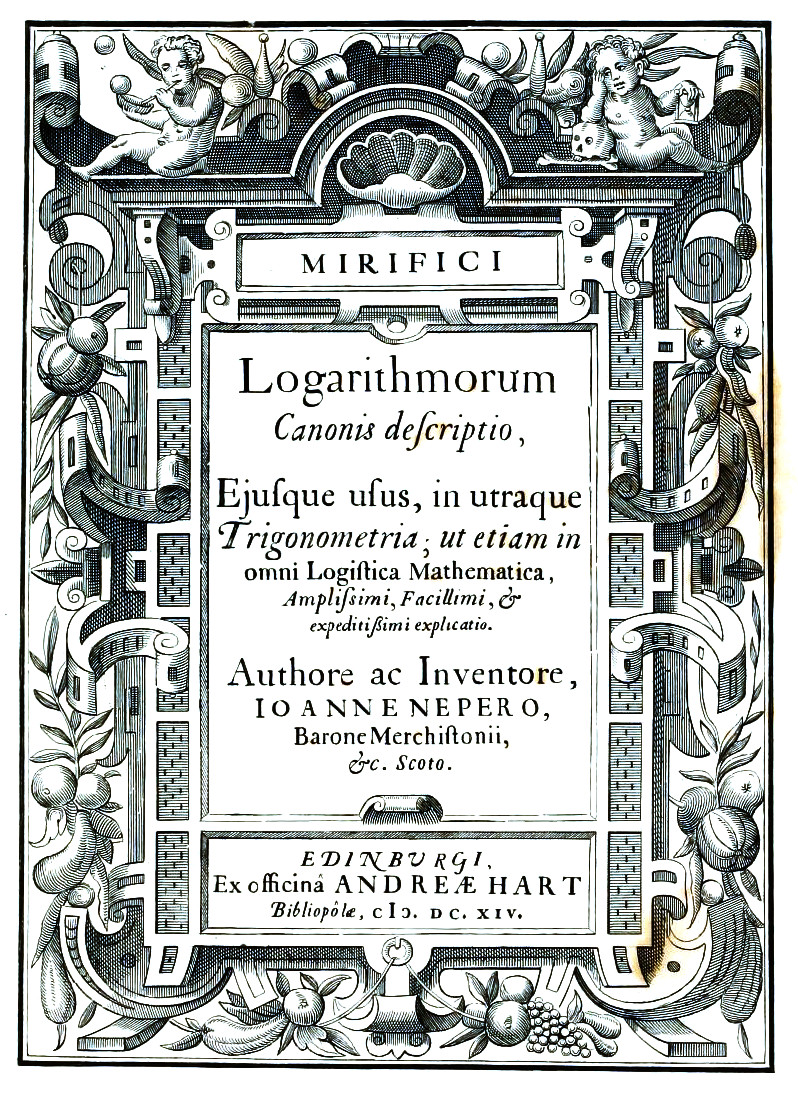
\includegraphics[width=1.75in]{Logarithms_book_Napier}
\end{minipage}
\hfil 
\begin{minipage}{0.7\textwidth}
    \begin{itemize}[nosep]
        \item Logarithms were invented before \gap{calculators}.
        \item They were a \gap{device} to make math calculations easier.
        \item Astronomy, geodesy, \dots
        \item trigonometry, spherical trignonometry, \dots
        \item John Napier (Scottish)
        \item Jost B{\"u}rgi (Swiss)
        \item Johannes Kepler (German)
        \item $\approx$ 1600
    \end{itemize}
\end{minipage}
\hfil 